% Provenance (never printed): old terminale S material on the Earth's internal
% heat (geothermal gradient and heat flow, radioactive heat production,
% conduction and convection, mantle convection, geothermal energy). Owner
% (Sync 0/1): heat flow, radiogenic heat production, secular cooling, thermal
% and mantle convection (recall the convection cell of Book 1 g8 first),
% geothermal energy. Geotherm and geothermal gradient are g11.03's; radioactivity,
% half-life, decay law and thermal conductivity are physics' (thermal
% conductivity used as "the rock's thermal conductivity k", never defined);
% hotspot track and plume g11.04's. Figures: figdata/grade-12/internal_heat.py.
\chapter{El calor interno de la Tierra}\label{ch:g12:internal-heat}

Entre 1987 y 1995, cerca del pueblo de Windischeschenbach, en Baviera, unos
geólogos perforaron un pozo de \qty{9101}{m} de profundidad en la \omterm{def:g12:continental-crust:continental-crust}{corteza
continental}. En el fondo, la roca estaba a unos \qty{265}{\celsius},
demasiado caliente para seguir perforando.
% ledger: gfz:ktb, gfz:ktb30

De unos \qty{10}{\celsius} en la superficie a \qty{265}{\celsius} a
\qty{9.1}{km} hay una subida de unos \qty{28}{\celsius} por kilómetro, un
valor típico. En todas partes de la Tierra hace más calor hacia abajo, así que
el calor sale de la Tierra continuamente. Este capítulo mide ese flujo, se
pregunta de dónde viene el calor y muestra cómo se desplaza.
% values: ktb_gradient 28.0 (internal_heat.py, surface temperature taken as 10 degC); ledger: gfz:ktb (gradient about 28 K/km)

\begin{recall}
La \omterm{def:g11:lithosphere-asthenosphere:geotherm}{geoterma} es la curva de la temperatura frente a la profundidad bajo un
lugar, y el \omterm{def:g11:lithosphere-asthenosphere:geotherm}{gradiente geotérmico}, la subida de la temperatura por kilómetro;
los sondeos miden de 25 a \qty{30}{\celsius} por kilómetro cerca de la
superficie (el \cref{ch:g11:lithosphere-asthenosphere}). Algunos átomos son
radiactivos: se desintegran al azar, el número de los que quedan se reduce a la
mitad en cada periodo de semidesintegración, y cada desintegración libera
energía, que acaba en forma de calor (los libros de física). Una celda de
convección es un circuito de fluido calentado desde abajo, que asciende, se
extiende, se enfría y se hunde (Libro 1, año 8). En un punto caliente, una
placa se desplaza sobre una pluma de manto caliente (el
\cref{ch:g11:plate-motions}).
\end{recall}
% ledger: usgs:gradient-29 (Book 1 row)

\section{Gradiente y flujo de calor}

\begin{definition}[Flujo de calor]\label{def:g12:internal-heat:heat-flow}
El \emph{flujo de calor}\index{flujo de calor} (o flujo térmico) en un lugar es
la potencia que sale del interior de la Tierra por cada metro cuadrado de su
superficie en ese lugar. Se mide en milivatios por metro cuadrado
(\unit{mW/m^2}).
\end{definition}
% ledger: b2dd10:continents

El calor fluye de lo caliente a lo frío, y cuanto más pronunciado es el
gradiente de temperatura, más deprisa fluye. Cuánto fluye depende también de
la roca: cada roca tiene una conductividad térmica $k$, en vatios por metro y
por kelvin, que definen los libros de física.

\begin{proposition}[Flujo de calor y gradiente]\label{prop:g12:internal-heat:fourier}
A través de una roca de conductividad térmica $k$ en la que la temperatura
aumenta con la profundidad según un gradiente $G$ (en kelvins por metro), el
\omterm{def:g12:internal-heat:heat-flow}{flujo de calor} hacia la superficie es
\[
  q = k\,G .
\]
\end{proposition}

Esta ley de la conducción, debida a Fourier, se admite aquí; los libros de
física la demuestran en una forma general.

\begin{method}[Un flujo de calor a partir de un sondeo]\label{met:g12:internal-heat:borehole}
\begin{enumerate}
  \item Mide la temperatura a varias profundidades de un sondeo, una vez que
        el pozo ha tenido tiempo de volver a la temperatura de la roca.
  \item Representa la temperatura frente a la profundidad y toma la
        pendiente: el gradiente $G$, convertido a kelvins por metro.
  \item Mide la conductividad $k$ de la roca en testigos, en el
        laboratorio.
  \item Multiplica: $q = kG$, en \unit{W/m^2}, y luego convierte a \unit{mW/m^2}.
\end{enumerate}
\end{method}

\begin{example}[Un sondeo en granito]\label{ex:g12:internal-heat:borehole}
Un sondeo en un granito de conductividad \qty{2.72}{W/(m.K)} mide un
gradiente de \qty{29}{\celsius} por kilómetro, es decir, \qty{0.029}{K/m}.
Entonces $q = 2.72 \times 0.029 \approx \qty{0.079}{W/m^2}$, unos
\qty{79}{mW/m^2}.
\end{example}
% ledger: roy:conductivity (granitic layer 6.5 mcal/(cm s degC) = 2.72 W/m/K), usgs:gradient-29 (Book 1 row)
% values: borehole_q_mW 78.9 (internal_heat.py)

Se han combinado más de 38\,000 medidas de este tipo en un mapa de toda la
Tierra. Los continentes pierden por término medio \qty{70.9}{mW/m^2}, el fondo
oceánico \qty{105.4}{mW/m^2}; sobre toda la superficie, \qty{91.6}{mW/m^2}.
Multiplicado por la superficie de la Tierra, \qty{5.101e14}{m^2}, el total es
\[
  0.0916 \times \num{5.101e14} \approx \qty{4.67e13}{W} = \qty{46.7}{TW},
\]
unos 47 teravatios, con un margen de 2.
% ledger: b2dd10:continents, b2dd10:half-space (47 +- 2 TW, 38,347 measurements)

El fondo oceánico pierde más donde es más joven. La \omterm{def:g11:lithosphere-asthenosphere:lithosphere}{litosfera} nueva sale
caliente de una dorsal y se enfría a medida que se aleja; su \omterm{def:g12:internal-heat:heat-flow}{flujo de calor}
disminuye como uno dividido por la raíz cuadrada de su edad.

\begin{omfigure}
\begin{tikzpicture}
\begin{axis}[omrecord, width=0.72\linewidth, height=5.6cm, xmin=0, xmax=180, ymin=0, ymax=400,
  xlabel={edad del fondo oceánico (millones de años)}, ylabel={flujo de calor (\unit{mW/m^2})},
  xtick={0,30,...,180}, ytick={0,100,...,400}]
% computed in figdata/grade-12/internal_heat.py; ledger: b2dd10:half-space, b2dd10:continents
\addplot[omDef, line width=1.1pt, restrict x to domain=0:66.5] table[x=t_Myr, y=q] {figdata/out/grade-12-internal_heat-halfspace.dat};
\addplot[omDef, line width=1.1pt, densely dotted, restrict x to domain=66.5:180] table[x=t_Myr, y=q] {figdata/out/grade-12-internal_heat-halfspace.dat};
\addplot[omProp, line width=0.9pt, dashed, domain=0:180] {70.9};
\coordinate (lawlab) at (axis cs:14,250);
\coordinate (contlab) at (axis cs:100,80);
\end{axis}
\node[font=\scriptsize, text=omDef, anchor=west] at (lawlab) {$q = 490/\sqrt{t}$};
\node[font=\scriptsize, text=omProp, anchor=south west] at (contlab) {media continental, \qty{70.9}{mW/m^2}};
\end{tikzpicture}

{\small \omterm{def:g12:internal-heat:heat-flow}{Flujo de calor} a través del fondo oceánico frente a su edad, calculado
para el enfriamiento de la \omterm{def:g11:lithosphere-asthenosphere:lithosphere}{litosfera} ($t$ en millones de años); más allá de
66.5 millones de años (punteado), se sabe que la ley se ajusta peor. Fuente:
Davies y Davies (2010).}
\end{omfigure}
% values: q_1Myr 490, q_10Myr 155, q_66.5Myr 60.1, age_where_q_equals_cont_Myr 47.8 (internal_heat.py)

\section{De dónde viene el calor}

El calor tiene dos fuentes. La primera es la radiactividad.

\begin{definition}[Producción de calor radiogénico]\label{def:g12:internal-heat:heat-production}
La \emph{producción de calor radiogénico}\index{produccion de calor radiogenico@producción de calor radiogénico}
de una roca es el calor que libera en su interior la desintegración de sus
átomos radiactivos, por unidad de volumen y de tiempo, en microvatios por
metro cúbico (\unit{\micro W/m^3}). Casi toda procede de cuatro isótopos: el
uranio 238, el uranio 235, el torio 232 y el potasio 40.
\end{definition}
% ledger: dye12:isotopes, earle:heat-sources, kamland11:geonu

Estos elementos están concentrados en las rocas de la \omterm{def:g12:continental-crust:continental-crust}{corteza continental}.
Según 2188 análisis, la producción de calor mediana del granito es de
\qty{2.43}{\micro W/m^3}, la del basalto de \qty{0.21}{\micro W/m^3}, y la de
las rocas ultramáficas del manto de solo \qty{0.11}{\micro W/m^3}, unas veinte
veces menos que el granito. Una capa de granito de \qty{10}{km} de espesor
produce
$2.43 \times 10^{-6} \times \num{10000} \approx \qty{0.024}{W}$ bajo cada
metro cuadrado, \qty{24}{mW/m^2}: un tercio del \omterm{def:g12:internal-heat:heat-flow}{flujo de calor} de los
continentes.
% ledger: b2vila:heat-production, b2dd10:continents
% values: granite_10km_mW 24.3, granite_over_ultramafic 21.9 (internal_heat.py)

¿Cuánto calor produce la radiactividad en toda la Tierra? KamLAND, un
detector subterráneo de Japón que contiene 1000 toneladas de líquido, capta
los geoneutrinos, los antineutrinos liberados por la desintegración del uranio
y el torio del interior de la Tierra: detectó los primeros en 2005 y, en 2135
días de registro, unos 106 de ellos entre 841 sucesos candidatos. A partir de
ese recuento, junto con el de un detector de Italia, el uranio 238 y el torio
232 liberan juntos unos 20 teravatios. El potasio 40 escapa al detector; se
sabe que añade unos \qty{4}{TW}, y el uranio 235, escalado a partir del
uranio 238, unos \qty{0.4}{TW}. La radiactividad aporta, pues, unos
\qty{24}{TW}, aproximadamente la mitad de los \qty{47}{TW} que pierde la
Tierra.
% ledger: kamland11:geonu, dye12:isotopes, b2dd10:continents
% values: now_K40_TW 4.0, now_U235_TW 0.42, radiogenic_TW 24.4, share_radiogenic 0.523 (internal_heat.py)

\begin{definition}[Enfriamiento secular]\label{def:g12:internal-heat:secular-cooling}
El \emph{enfriamiento secular}\index{enfriamiento secular} de la Tierra es la
lenta pérdida del calor almacenado en su interior desde que se formó, el
calor primordial: la parte del \omterm{def:g12:internal-heat:heat-flow}{flujo de calor} que la radiactividad no
repone, por la que el manto y el núcleo se van enfriando con las eras.
\end{definition}
% ledger: kamland11:geonu, earle:heat-sources

\begin{omfigure}
\begin{tikzpicture}
\begin{axis}[omrecord, xbar stacked, bar width=14pt, width=0.66\linewidth, height=3.2cm, scale only axis,
  xmin=0, xmax=50, ymin=0.4, ymax=2.6, ytick={1,2}, yticklabels={{fuentes}, {pérdidas}},
  xlabel={potencia (\unit{TW})}, ymajorgrids=false, legend columns=2, legend cell align=left,
  legend style={font=\scriptsize, at={(0.5,-0.42)}, anchor=north, /tikz/every even column/.append style={column sep=6pt}}]
% computed in figdata/grade-12/internal_heat.py; ledger: kamland11:geonu, dye12:isotopes, b2dd10:continents
\addplot[fill=omThm!55, draw=omThm] table[x=uth, y=bar] {figdata/out/grade-12-internal_heat-budget.dat};
\addplot[fill=omThm!25, draw=omThm] table[x=kuf, y=bar] {figdata/out/grade-12-internal_heat-budget.dat};
\addplot[fill=omDef!35, draw=omDef] table[x=secular, y=bar] {figdata/out/grade-12-internal_heat-budget.dat};
\addplot[fill=black!25, draw=black!60] table[x=surface, y=bar] {figdata/out/grade-12-internal_heat-budget.dat};
\legend{{uranio 238 y torio 232 (geoneutrinos)}, {potasio 40 y uranio 235}, {enfriamiento secular (el resto)}, {flujo de calor en la superficie}}
\end{axis}
\end{tikzpicture}

{\small El balance de calor de la Tierra hoy: lo que sale por la superficie
(barra de arriba) y lo que lo aporta (barra de abajo). Fuentes: KamLAND
(2011); Davies y Davies (2010); Dye (2012).}
\end{omfigure}
% values: radiogenic_TW 24.4, secular_TW 22.3 (internal_heat.py)

La radiactividad era más intensa en el pasado. Cada isótopo se desintegra,
así que hace mucho había más: un periodo de semidesintegración atrás, el
doble, y el doble de calor. Retroceder $t$ años multiplica el calor de un
isótopo de periodo de semidesintegración $T$ por $2^{t/T}$.

\begin{proposition}[El calor radiogénico en el pasado]\label{prop:g12:internal-heat:past}
Si un isótopo de periodo de semidesintegración $T$ libera hoy una potencia $H_0$, liberaba
\[
  H(t) = H_0 \, 2^{t/T} = H_0\, e^{\lambda t}, \qquad \lambda = \frac{\ln 2}{T},
\]
hace un tiempo $t$.
\end{proposition}

\begin{proof}
La potencia es proporcional al número $N$ de átomos que quedan, ya que cada
uno se desintegra con la misma probabilidad por segundo. Según la ley de
desintegración, $N$ se divide por 2 en cada periodo de semidesintegración: $N_{\text{hoy}} = N(t)\,2^{-t/T}$, así que $N(t) =
N_{\text{hoy}}\,2^{t/T}$, y de ahí se sigue la potencia. Por último, $2^{t/T} =
e^{(t/T)\ln 2} = e^{\lambda t}$.
\end{proof}

\begin{omfigure}
\begin{tikzpicture}
\begin{axis}[omrecord, width=0.72\linewidth, height=6cm, xmin=0, xmax=4.5, ymin=0, ymax=120,
  x dir=reverse, xlabel={tiempo antes del presente (miles de millones de años)}, ylabel={calor radiogénico (\unit{TW})},
  xtick={0,0.5,...,4.5}, ytick={0,20,...,120}, x tick label style={/pgf/number format/.cd, fixed, precision=1},
  legend pos=north east, legend style={font=\scriptsize}, legend cell align=left]
% computed in figdata/grade-12/internal_heat.py; ledger: kamland11:geonu, dye12:isotopes, nndc:halflives
\addplot[black, line width=1.2pt] table[x=t_Ga, y=total] {figdata/out/grade-12-internal_heat-past.dat};
\addplot[omThm, line width=0.9pt] table[x=t_Ga, y=U235] {figdata/out/grade-12-internal_heat-past.dat};
\addplot[omProp, line width=0.9pt, densely dashed] table[x=t_Ga, y=K40] {figdata/out/grade-12-internal_heat-past.dat};
\addplot[omDef, line width=0.9pt] table[x=t_Ga, y=U238] {figdata/out/grade-12-internal_heat-past.dat};
\addplot[omMeth, line width=0.9pt, densely dotted] table[x=t_Ga, y=Th232] {figdata/out/grade-12-internal_heat-past.dat};
\legend{total, uranio 235, potasio 40, uranio 238, torio 232}
\end{axis}
\end{tikzpicture}

{\small El calor liberado por los cuatro isótopos radiactivos desde la
formación de la Tierra, calculado a partir de los valores actuales con la ley
de desintegración. Periodos de semidesintegración: torio 232, 14\,000 millones
de años; uranio 238, 4468 millones; potasio 40, 1248 millones; uranio 235, 704
millones.}
\end{omfigure}
% values: total_4.5Ga_TW 115.9, ratio_total_4.5Ga 4.75, ratio_U235_4.5Ga 84.0, ratio_K40_4.5Ga 12.2, share_U235_K40_4.5Ga 0.72 (internal_heat.py)

Hace cuatro mil quinientos millones de años, la radiactividad liberaba unos
\qty{116}{TW}, casi cinco veces el valor actual, y la mayor parte procedía del
uranio 235 y del potasio 40, los dos isótopos de vida corta, que desde
entonces casi han desaparecido. La Tierra joven estaba por dentro mucho más
caliente que hoy.
% ledger: earle:heat-sources (radiogenic heat now roughly 25 % of what it was)

\section{Conducción y convección}

El calor solo puede atravesar un sólido por conducción, de átomo en átomo, y
en la roca eso es muy lento. El calor atraviesa por conducción una distancia
$L$ en un tiempo de unos $L^2/\kappa$, donde $\kappa$, la difusividad térmica
de la roca, es de unos \qty{1e-6}{m^2/s}. Para los
\qty{2891}{km} del manto,
\[
  \frac{(\num{2.891e6})^2}{\num{1e-6}} \approx \qty{8.4e18}{s} \approx
  \num{2.6e11} \text{ años},
\]
unos 260\,000 millones de años, casi sesenta veces la edad de la Tierra. Si el
manto solo condujera el calor, el calor de sus profundidades seguiría casi
todo allí.
% ledger: england:kelvin (Book 3 row: kappa 1e-6 m2/s), data:prem (CMB at 2891 km)
% values: conduction_time_Gyr 264.9 (internal_heat.py)

El manto es sólido, pero a lo largo de millones de años repta, muy despacio,
como un fluido muy rígido: la \omterm{def:g11:lithosphere-asthenosphere:lithosphere}{astenosfera} fluye (el
\cref{ch:g11:lithosphere-asthenosphere}). Así que el manto pierde su calor como
el aire que hay sobre un radiador: transportándolo.

\begin{definition}[Convección térmica; convección del manto]\label{def:g12:internal-heat:convection}
La \emph{convección térmica}\index{conveccion termica@convección térmica} es el
transporte de calor por el movimiento del propio material: el material más
caliente y ligero asciende, y el más frío y denso se hunde, como en una celda
de convección. La \emph{convección del manto}\index{conveccion del manto@convección del manto}
es la convección térmica del manto sólido de la Tierra, que repta a unos
pocos centímetros al año y lleva el calor del interior hacia la superficie.
\end{definition}
% ledger: earle:heat-sources (solid mantle flows at centimetres a year)

Las placas son la parte superior de esta convección. En las dorsales, el
manto caliente asciende y se añade a las placas; la \omterm{def:g11:lithosphere-asthenosphere:lithosphere}{litosfera} se enfría a
medida que se aleja, se vuelve densa y se hunde por su propio peso en las
\omterm{def:g11:subduction-zones:subduction}{zonas de subducción}: las \omterm{def:g11:subduction-zones:slab}{losas} son la parte fría y descendente del flujo, y
las imágenes sísmicas las muestran hundiéndose hasta muy hondo en el manto. Se
cree que bajo los puntos calientes ascienden plumas de roca caliente desde lo
profundo del manto, quizá desde justo encima del núcleo.
% ledger: dye12:bse, earle:plume

\begin{omfigure}
\begin{tikzpicture}[x=1cm, y=1cm, font=\scriptsize]
  % mantle annulus sector
  \fill[omLithPeridotite!40] (0,0) ++(20:6.4) arc (20:160:6.4) -- ++(160:-3.2) arc (160:20:3.2) -- cycle;
  \fill[black!45] (0,0) ++(20:3.2) arc (20:160:3.2) -- (0,0) -- cycle;
  \node[white] at (0,1.6) {núcleo};
  % lithosphere
  \fill[black!15, draw=black!50] (0,0) ++(20:6.4) arc (20:160:6.4) -- ++(160:-0.3) arc (160:20:6.1) -- cycle;
  % ridge (top) and two trenches
  \draw[omThm, line width=1pt, -{Stealth}] (0,5.9) -- (0,6.35);
  \node[anchor=south] at (0,6.45) {dorsal};
  \foreach \a/\lab in {48/fosa, 132/fosa} {
    \node[anchor=south] at (\a:6.5) {\lab};
  }
  % slabs (cold, blue) sinking from the trenches
  \draw[omDef, line width=3pt] (48:6.2) .. controls (52:5.2) and (60:4.4) .. (62:3.4);
  \draw[omDef, line width=3pt] (132:6.2) .. controls (128:5.2) and (120:4.4) .. (118:3.4);
  % plume (hot, red) rising
  \draw[omThm, line width=2.4pt] (155:3.25) .. controls (154:4.2) and (152:5.2) .. (151:6.05);
  \fill[omThm] (151:6.0) circle (0.18);
  \node[anchor=west, text=omThm] at (145:4.0) {¿pluma?};
  % convection arrows
  \draw[-{Stealth}, black!65, line width=0.8pt] (80:5.7) arc (80:58:5.7);
  \draw[-{Stealth}, black!65, line width=0.8pt] (100:5.7) arc (100:122:5.7);
  \draw[-{Stealth}, black!65, line width=0.8pt] (68:3.7) .. controls (80:3.6) and (88:4.5) .. (90:5.4);
  \draw[-{Stealth}, black!65, line width=0.8pt] (112:3.7) .. controls (100:3.6) and (92:4.5) .. (90:5.4);
  \node[omDef, anchor=north west, align=left] at (52:4.55) {la losa fría\\se hunde};
  \node[anchor=north, white] at (90:2.95) {límite núcleo--manto};
  \node[anchor=south east] at (150:6.45) {placas};
\end{tikzpicture}

{\small La \omterm{def:g12:internal-heat:convection}{convección del manto} (esquema, sin escala). Las placas son su
límite superior frío: el manto caliente asciende bajo las dorsales, y las
placas se enfrían a medida que se alejan y se hunden de nuevo en forma de
\omterm{def:g11:subduction-zones:slab}{losas} en las fosas, algunas hasta el manto inferior. Bajo los puntos calientes
pueden ascender plumas desde gran profundidad.}
\end{omfigure}
% ledger: dye12:bse, earle:plume

Así, la mayor parte del calor sale del manto por convección, y solo las
últimas decenas de kilómetros, a través de la \omterm{def:g11:lithosphere-asthenosphere:lithosphere}{litosfera} rígida, se atraviesan
por conducción: la conducción que miden los sondeos.
% ledger: dye12:bse (convection the main transport of interior heat), earle:heat-sources

\section{La energía geotérmica}

\begin{definition}[Energía geotérmica]\label{def:g12:internal-heat:geothermal}
La \emph{energía geotérmica}\index{energia geotermica@energía geotérmica} es el calor
del interior de la Tierra que aprovecha el ser humano: agua caliente o vapor
procedentes de roca caliente, extraídos por pozos para calefacción o para
producir electricidad.
\end{definition}
% ledger: eia:geo-use, eia:geo-plants

El calor que sale de la Tierra es minúsculo allí donde llega a la superficie,
unos \qty{0.1}{W} bajo cada metro cuadrado, demasiado poco para aprovecharlo
directamente. Se vuelve aprovechable donde se concentra a poca profundidad.
Cerca de los volcanes, los rifts y los puntos calientes, y a lo largo de los
límites de placas, la roca caliente se acerca a la superficie, y el agua que
circula por la roca permeable vuelve caliente. Una central eléctrica necesita
agua muy caliente o vapor, de unos 150 a \qty{370}{\celsius}; algunos campos
dan vapor seco, que mueve directamente las turbinas. La primera electricidad
obtenida del calor de la Tierra se produjo en 1904 en Larderello, en la
Toscana: encendió cinco bombillas. En otros lugares, el agua caliente de poca
profundidad se lleva por tuberías a los edificios para calentarlos.
% ledger: b2dd10:continents, eia:geo-where, eia:geo-plants (300 to 700 degF), enel:larderello, eia:geo-use

\begin{omfigure}
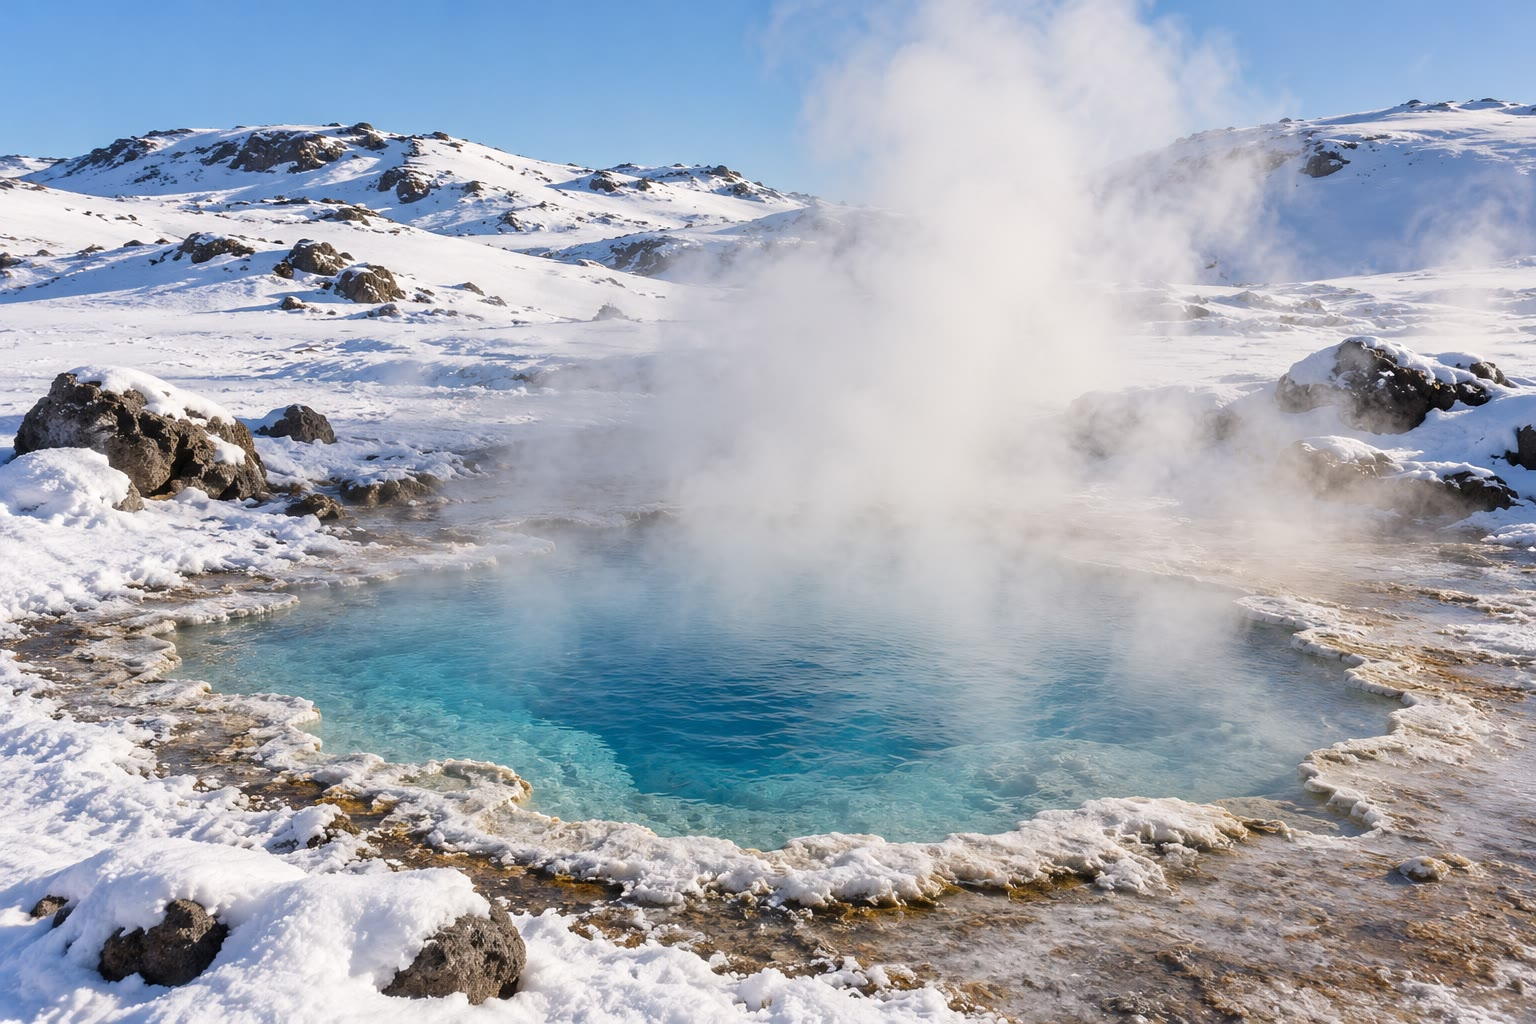
\includegraphics[width=0.6\linewidth]{images/book2/ai/g12-hot-spring-snow.jpg}

{\small Una fuente termal humeante en un paisaje nevado: agua calentada en lo
profundo del subsuelo vuelve a la superficie. Ilustración generada por IA.}
\end{omfigure}

\begin{omfigure}
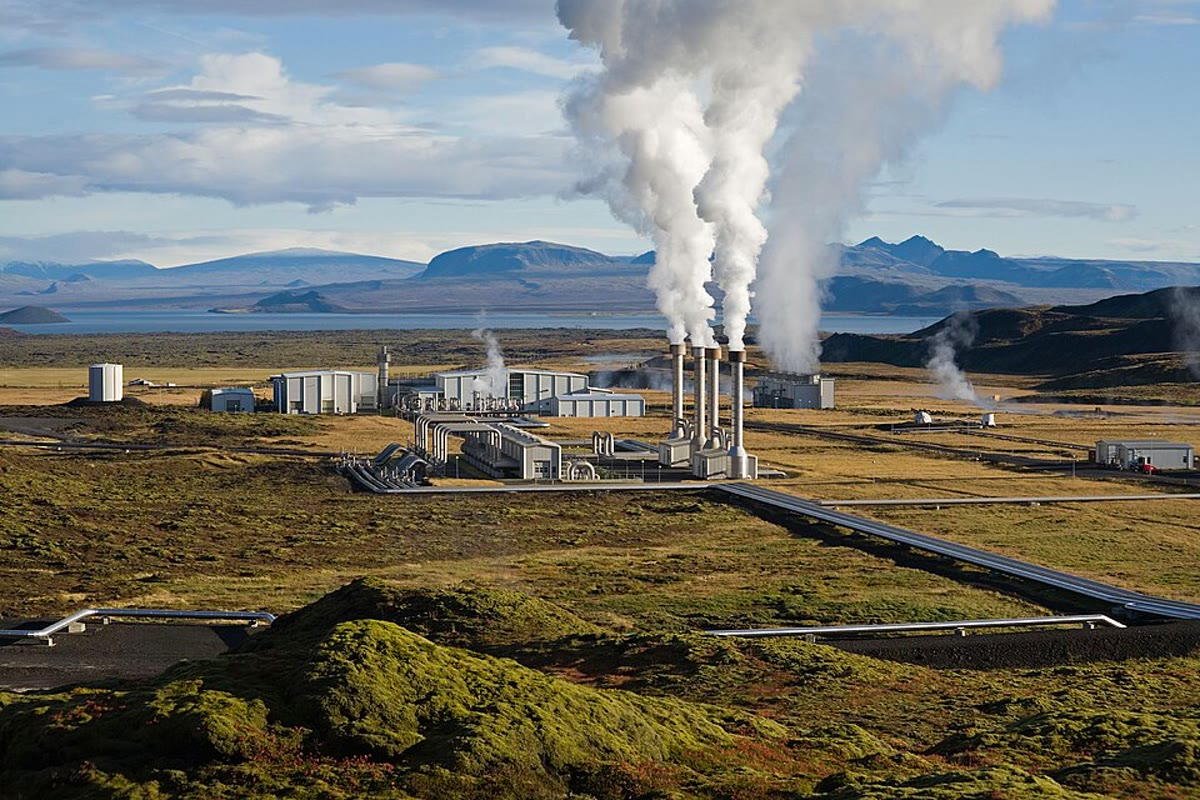
\includegraphics[width=0.66\linewidth]{images/book2/g12-nesjavellir-geothermal.jpg}

{\small La central geotérmica de Nesjavellir, en la zona volcánica de Hengill,
Islandia: hasta \qty{120}{MW} de electricidad y hasta \qty{300}{MW} de calor,
transportado por agua caliente. Fotografía de Gretar Ívarsson (dominio
público).}
\end{omfigure}
% ledger: photo:g12-nesjavellir, on:nesjavellir

Un campo geotérmico no es inagotable a la escala de una vida humana. En The
Geysers, en California, demasiados pozos extrajeron el vapor más deprisa de
lo que el lento \omterm{def:g12:internal-heat:heat-flow}{flujo de calor} y la lluvia podían reponerlo: la presión del
vapor cayó a menos de la mitad de su máximo, y se perdió más del
\qty{40}{\percent} de la capacidad de las centrales. Hoy se vuelve a inyectar
agua en el campo para frenar el declive.
% ledger: cpuc:geysers

\section{Ejercicios}

\begin{exercise}[$\star$]\label{exo:g12:internal-heat:1}
Da la palabra: (a) la potencia que sale del interior por cada metro cuadrado
de superficie; (b) el calor liberado por la desintegración de los átomos
radiactivos en una unidad de volumen de roca; (c) la pérdida del calor
almacenado desde que se formó la Tierra; (d) el transporte de calor por el
movimiento del propio material; (e) el calor interno de la Tierra que
aprovecha el ser humano.
\end{exercise}

\begin{exercise}[$\star$]\label{exo:g12:internal-heat:2}
Convierte: (1) \qty{91.6}{mW/m^2} en \unit{W/m^2}; (2) \qty{46.7}{TW} en
vatios; (3) \qty{29}{\celsius} por kilómetro en kelvins por metro.
\end{exercise}

\begin{exercise}[$\star$]\label{exo:g12:internal-heat:3}
Nombra los cuatro isótopos que producen casi todo el calor radiogénico, y di
cuáles dos puede ver el detector KamLAND.
\end{exercise}

\begin{exercise}[$\star$]\label{exo:g12:internal-heat:4}
Con $q = 490/\sqrt{t}$, calcula el \omterm{def:g12:internal-heat:heat-flow}{flujo de calor} a través de un fondo
oceánico de 1, 4, 25 y 49 millones de años.
\end{exercise}

\begin{exercise}[$\star$]\label{exo:g12:internal-heat:5}
¿Por qué el \omterm{def:g12:internal-heat:heat-flow}{flujo de calor} se mide en sondeos y no en la propia superficie?
¿Por qué hay que esperar tras la perforación antes de medir?
\end{exercise}

\begin{exercise}[$\star\star$]\label{exo:g12:internal-heat:6}
En el sondeo KTB, la roca estaba a unos \qty{265}{\celsius} a
\qty{9.1}{km}. (1) Tomando \qty{10}{\celsius} en la superficie, calcula el
gradiente medio. (2) Con una conductividad de \qty{2.72}{W/(m.K)}, ¿qué \omterm{def:g12:internal-heat:heat-flow}{flujo
de calor} da? (3) Compáralo con la media de los continentes.
\end{exercise}

\begin{exercise}[$\star\star$]\label{exo:g12:internal-heat:7}
Los continentes cubren \qty{2.073e14}{m^2} con un \omterm{def:g12:internal-heat:heat-flow}{flujo de calor} medio de
\qty{70.9}{mW/m^2}, y los océanos \qty{3.028e14}{m^2} con
\qty{105.4}{mW/m^2}. Calcula la potencia que pierde cada uno, el total y la
fracción que se pierde a través del fondo oceánico.
\end{exercise}

\begin{exercise}[$\star\star$]\label{exo:g12:internal-heat:8}
Una capa de \omterm{def:g12:subduction-magmatism:granodiorite}{granodiorita} de \qty{8}{km} de espesor tiene una producción de
calor de \qty{1.88}{\micro W/m^3}. (1) ¿Qué \omterm{def:g12:internal-heat:heat-flow}{flujo de calor} produce en la
superficie? (2) ¿Qué fracción es de \qty{70.9}{mW/m^2}?
\end{exercise}

\begin{exercise}[$\star\star$]\label{exo:g12:internal-heat:9}
¿A qué edad pierde el fondo oceánico tanto calor como el continente medio,
\qty{70.9}{mW/m^2}, según $q = 490/\sqrt{t}$?
\end{exercise}

\begin{exercise}[$\star\star$]\label{exo:g12:internal-heat:10}
¿Cuánto más calor liberaba el uranio 235 hace 1400 millones de años que hoy?
¿Y el potasio 40 hace 2500 millones de años?
\end{exercise}

\begin{exercise}[$\star\star$]\label{exo:g12:internal-heat:11}
Con $t \approx L^2/\kappa$ y $\kappa = \qty{1e-6}{m^2/s}$, ¿cuánto tarda el
calor en atravesar por conducción (1) una colada de lava de \qty{10}{m} de
espesor; (2) una \omterm{def:g11:lithosphere-asthenosphere:lithosphere}{litosfera} de \qty{100}{km} de espesor; (3) el manto? Expresa
cada resultado en unidades razonables.
\end{exercise}

\begin{exercise}[$\star\star\star$]\label{exo:g12:internal-heat:12}
Hoy, el torio 232 libera unos \qty{10.4}{TW}, el uranio 238 \qty{9.6}{TW},
el potasio 40 \qty{4.0}{TW} y el uranio 235 \qty{0.42}{TW}. Con los periodos
de semidesintegración de la figura, calcula el calor de
cada uno hace 3000 millones de años, el total y la fracción de los dos
isótopos de vida corta.
\end{exercise}

\begin{exercise}[$\star\star\star$]\label{exo:g12:internal-heat:13}
La central de Nesjavellir puede suministrar hasta \qty{300}{MW} de calor,
transportados por unos \qty{1640}{L} de agua caliente por segundo. Con un
calor específico de \qty{4180}{J/(kg.K)} y una masa de \qty{1}{kg} por litro,
¿cuántos grados se ha calentado esta agua? ¿Qué superficie de continente medio
pierde \qty{300}{MW} de calor?
\end{exercise}

\begin{exercise}[$\star\star\star$]\label{exo:g12:internal-heat:14}
Supón que una placa tarda 100 millones de años en ir de una dorsal a una fosa,
y un circuito de convección por todo el manto unos 200 millones de años. (1)
Compara estos tiempos con los 260\,000 millones de años de la conducción a
través del manto. (2) ¿Por qué la convección puede transportar el calor
mucho más deprisa, aunque el manto solo se mueva unos centímetros al año?
\end{exercise}

\begin{exercise}[$\star\star\star$]\label{exo:g12:internal-heat:15}
Supón que el núcleo pierde unos \qty{10}{TW} de calor hacia el manto a
través del \omterm{def:g11:seismic-structure:core}{límite núcleo--manto}, a \qty{2891}{km} de profundidad. (1) ¿Qué
fracción del \omterm{def:g12:internal-heat:secular-cooling}{enfriamiento secular}, \qty{22.3}{TW}, sería? ¿De dónde viene el
resto? (2) Calcula el \omterm{def:g12:internal-heat:heat-flow}{flujo de calor} medio a través del
\omterm{def:g11:seismic-structure:core}{límite núcleo--manto}, y compáralo con el \omterm{def:g12:internal-heat:heat-flow}{flujo de calor} medio en la superficie,
\qty{91.6}{mW/m^2}. (3) ¿Por qué el núcleo caliente puede calentar la base
del manto aunque el manto sea sólido?
\end{exercise}

\begin{problem}[{Problema de fin de semana --- El balance de calor de la Tierra}]
\label{pb:g12:internal-heat:1}
% ledger: b2dd10:continents, b2dd10:half-space, kamland11:geonu, dye12:isotopes, dye12:bse, b2vila:heat-production
% values (internal_heat.py): radiogenic 24.4 TW, secular 22.3 TW, share 0.523, K40 4.0, U235 0.42, U238 9.59
El \omterm{def:g12:internal-heat:heat-flow}{flujo de calor} de la Tierra se ha medido en más de 38\,000 lugares. Por
término medio, los continentes pierden \qty{70.9}{mW/m^2} sobre
\qty{2.073e14}{m^2}, y el fondo oceánico \qty{105.4}{mW/m^2} sobre
\qty{3.028e14}{m^2}.

\medskip
\noindent\textbf{Parte I --- Flujo de calor y superficies.}
\begin{enumerate}
  \item Comprueba que las dos superficies suman la superficie de una esfera
        de \qty{6371}{km} de radio.
  \item ¿Qué fracción de la superficie es fondo oceánico?
  \item ¿Por qué el fondo oceánico pierde más calor por metro cuadrado que los
        continentes?
  \item Con $q = 490/\sqrt{t}$, calcula el \omterm{def:g12:internal-heat:heat-flow}{flujo de calor} a través de un
        fondo oceánico de 4 millones de años.
  \item Un sondeo en granito (\qty{2.72}{W/(m.K)}) mide \qty{26}{\celsius}
        por kilómetro. ¿Está su \omterm{def:g12:internal-heat:heat-flow}{flujo de calor} por encima o por debajo de la
        media continental?
\end{enumerate}

\medskip
\noindent\textbf{Parte II --- El total.}
\begin{enumerate}[resume]
  \item Calcula la potencia que se pierde a través de los continentes.
  \item Calcula la potencia que se pierde a través del fondo oceánico.
  \item Súmalas: el \omterm{def:g12:internal-heat:heat-flow}{flujo de calor} total de la Tierra, en teravatios.
  \item ¿Cuál es el \omterm{def:g12:internal-heat:heat-flow}{flujo de calor} medio sobre toda la superficie?
  \item Si bajo cada continente hubiera \qty{10}{km} de granito
        (\qty{24.3}{mW/m^2}), ¿cuántos teravatios produciría? Compáralo con la
        potencia que se pierde a través de los continentes.
\end{enumerate}

\medskip
\noindent\textbf{Parte III --- El calor radiogénico.}
\begin{enumerate}[resume]
  \item KamLAND cuenta los geoneutrinos del uranio 238 y del torio 232: juntos
        liberan unos \qty{20.0}{TW}, con \qty{3.9}{kg} de torio en la Tierra
        por cada kilogramo de uranio. Un kilogramo de uranio libera
        \qty{94.4}{\micro W} con su uranio 238 y \qty{4.10}{\micro W} con su
        uranio 235; un kilogramo de torio, \qty{26.3}{\micro W}. Calcula el
        calor del uranio 238 y luego el del uranio 235.
  \item El potasio 40 añade unos \qty{4}{TW}. Calcula el calor radiogénico total.
  \item ¿Qué tipo de roca lleva la mayor parte de estos elementos, y dónde está?
  \item ¿Era el calor radiogénico mayor o menor hace 3000 millones de años? ¿Por qué?
\end{enumerate}

\medskip
\noindent\textbf{Parte IV --- El enfriamiento secular.}
\begin{enumerate}[resume]
  \item ¿Qué potencia no aporta la radiactividad?
  \item ¿De dónde procede?
  \item Calcula la fracción del \omterm{def:g12:internal-heat:heat-flow}{flujo de calor} que aporta el \omterm{def:g12:internal-heat:secular-cooling}{enfriamiento secular}.
  \item Los modelos de la composición de la Tierra dan un calor radiogénico de
        11 a \qty{38}{TW}.
        ¿Entre qué fracciones se encuentra entonces la parte radiogénica?
  \item ¿Qué transporta la mayor parte de este calor a través del manto?
  \item En resumen: ¿qué fracción de la pérdida de calor de la Tierra aporta
        hoy la radiactividad?
\end{enumerate}
\end{problem}
